\chapter{Results}
\label{sec:results}

In this chapter, results of GAT-Denoiser are presented.
First, the LoDoPaB-CT dataset is introduced, and some illustrations are given.
Second, the project setup and shared settings are given.
Third, small scale GAT-Denoiser experiments are presented, where the goal is to find
good parameters for training the GAT-Denoiser model.
Last, the large scale GAT-Denoiser experiments are presented, where the goal is 
to find the best model.



\section{Dataset}
GAT-Denoiser is tested on the LoDoPaB-CT~\cite{lodopab-dataset} dataset, which is a 
benchmark dataset for low-dose CT reconstruction methods and therefore well suited for our domain.

The dataset consists of 35'820 train images and 3'553 test images.
All these images are having resolution 64x64.

\begin{figure}[H]
  \centering
  \hfill
  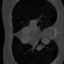
\includegraphics[width=0.2\textwidth]{ct_im_0.png}
  \hfill
  
\includegraphics[width=0.2\textwidth]{ct_im_1.png}
  \hfill
  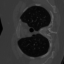
\includegraphics[width=0.2\textwidth]{ct_im_2.png}
  \hfill
  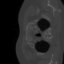
\includegraphics[width=0.2\textwidth]{ct_im_3.png}
  \hfill
  \caption{Some training images of LoDoPaB-CT dataset.}
\end{figure}



\section{Project Setup}
Python source code of the project is available on GitHub\footnote{https://github.com/cedricmendelin/master-thesis}.
Several python packages are used in the code and the most important one are listed: Pytorch geometric\footnote{https://pytorch-geometric.readthedocs.io/en/latest/} 
for neural network configuration, Operator Discretization Library\footnote{https://odlgroup.github.io/odl/} for Radon Transform and FBP, 
and last, Weight \& Bias\footnote{https://wandb.ai/site} (wandb) to gather results in a convenient way.

Training of GAT-Denoiser has been performed on the HPC-cluster scicore of the University of Basel.
During training, up to 4 titanx GPUs with each 12 GB RAM have been used.


\paragraph{Radon Transform:}
For Radon Transform, sampling points have been fixed to 64, thus $s \in \mathbb{R}^{64}$.
Further, projection angles $\theta$ are sampled within interval $[0, \pi]$.
The number of observation is the size of our input graph nodes, where typically 1024 are used.

\paragraph{GAT settings:}
During experiments, in the GAT layers exponential linear unit (ELU) was used as an activation function.
Further, dropout is used as regularization term.
During training, Adam~\cite{adam} optimizer was applied with learning rate $0.01$ and weight decay $0.0005$.
Moreover, mini batch gradient descent with a batch size of 64 was computed.

\paragraph{Performance metrics:}
During evaluation, two main metrics are considered.
First, \textit{Loss} is used, which refers to the average $\ell$-2 distance between the biological sample and reconstruction.
Second, \textit{SNR} is used, which refers to SNR in dB of reconstruction, compared to the biological sample.
Further, visual results are presented and can be seen as a third metric.


\paragraph{U-Net training:}
U-Net was pre-trained on the LoDoPaB-CT training dataset, with 128 channels in the first contracting step. 
In total, 4 steps have been computed, which results in 1024 channels as output of last contracting step.
During training, noise was sampled from normal distribution to reach SNR in the interval $[0, -10]$ dB 
and was added to the observation. In total, the model was trained for 200 epochs.

\paragraph{BM3D:}
In the GAT-Denoiser pipeline, first, observations will be denoised, and second, reconstruction is computed.
Therefore, BM3D can be applied at two different steps. First, it can be used to denoise sinogram
and forward denoised sinogram to FBP, which is how GAT-Denoiser work. Secondly, FBP can be
computed with noisy sinogram and output can be forwarded to BM3D, which will denoise reconstruction.
In the following term \textit{BM3D sino} and \textit{BM3D reco} are used to distinguish between the two approaches.

\section{Small Scale GAT-Denoiser Experiments}
For small scale experiments, not the complete LoDoPaB-CT dataset was considered, but only 1024 train images
and 100 validation images. 
Further, evaluated GAT-Denoiser models presented in this section have been trained for 200 epochs.

\subsection{Baseline}

Table~\ref{tab:baseline-small} shows baseline results for FBP, BM3D sino, BM3D reco and U-Net.
Noise was added to reach \snry of 0, -5, -10 and -15 dB.

As expected, reconstruction with FBP performs the worst, as it only reconstructs from noisy observation.
BM3D-sino and BM3D-reco perform surprisingly good for higher $\textit{SNR}_y$.
Although, for lower \snry the algorithm performs poorly as well.

Figure~\ref{fig:baseline_small} illustrates the reconstruction of a single
observation for all baseline algorithms. \snry is set to 0 dB.

Visually U-Net reconstruction looks best, but the SNR was lower compared to the BM3D approaches.
After some investigation, a small bug in the pre-trained U-Net model was found.
There was an issue with the amplitude of U-Net reconstruction,
therefore the SNR values of U-Net are expected to be slightly higher.
But also the pre-trained U-Net model starts to fail reconstruction with lower \snry.


\begin{table}[H]
  \centering
  \begin{tabular}{l|cc|cc|cc|cc}
    \toprule
    \textbf{Algorithm} & \multicolumn{2}{c|}{\snrh{ 0}} & \multicolumn{2}{c|}{\snrh{ -5}} & \multicolumn{2}{c|}{\snrh{ -10}} & \multicolumn{2}{l}{\snrh{ -15}} \\
                       & \textbf{SNR} & \textbf{Loss}  & \textbf{SNR} & \textbf{Loss}  & \textbf{SNR} & \textbf{Loss} & \textbf{SNR} & \textbf{Loss} \\ 
    \midrule
    FBP                 & 4.50 & 1182.3 & -0.31 & 1982.2 & -5.25 & 3454.1 & -10.22 & 6101.7 \\ \hline
    BM3D-sino           & 9.93 & 714.2 &  7.42 & 892.2 & 4.61 & 1179.8 & 2.00 & 1570.1 \\ \hline
    BM3D-reco           & 10.79 & 664.5 & 8.09 & 833.6 & 4.97 & 1137.7 & 1.54 & 1677.5 \\ \hline
    U-Net               & 7.13 & 977.7 &  6.18 & 1054.1 & 4.34 & 1235.0 & 1.87 & 1545.4 \\ \hline
    \midrule
  \end{tabular}

  \caption{Baseline results small experiments: the best result in column is marked bold. }
  \label{tab:baseline-small}
\end{table}




\begin{figure}[H]
  \captionsetup[subfigure]{justification=centering}
  \centering
  \begin{subfigure}[t]{0.15\textwidth}
      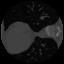
\includegraphics[width=\textwidth]{baseline_small_clean.png}
      \caption{Clean image}
  \end{subfigure}\hfill
  \begin{subfigure}[t]{0.15\textwidth}
    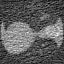
\includegraphics[width=\textwidth]{baseline_small_fbp.png}
    \caption{FBP reconstruction}
  \end{subfigure}\hfill
  \begin{subfigure}[t]{0.15\textwidth}
    
\includegraphics[width=\textwidth]{baseline_small_bm3d_sino.png}
    \caption{BM3D sino reconstruction}
  \end{subfigure}\hfill
  \begin{subfigure}[t]{0.15\textwidth}
    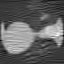
\includegraphics[width=\textwidth]{baseline_small_bm3d_reco.png}
    \caption{BM3D reco reconstruction}
  \end{subfigure}\hfill
  \begin{subfigure}[t]{0.15\textwidth}
    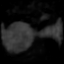
\includegraphics[width=\textwidth]{baseline_small_unet.png}
    \caption{U-Net reconstruction}
  \end{subfigure}
  \caption{Sample reconstruction for baseline algorithms and \snry 0 dB}
  \label{fig:baseline_small}
\end{figure}


 \subsection{K-NN Experiments}
  In the following section, experiments with different input graphs are presented.
  Therefore, some other parameters are fixed for all experiments.
  First, U-Net was deactivated, resulting reconstruction is defined as FBP solely.
  Further, GAT-Denoiser has been set to 3 layers with GAT single head and convolution 
  with one channel, kernel size 3 and padding 1. 
  If nothing else noted, noise was added to reach \snry 0 dB.

  The input graph structure is important for GAT learning.
  In our case, GL embedding for the observation is expected to be a circle and therefore,
  the input graph was fixed. A k-NN graph was built from angles, which are mapped to
  the unit-circle and great-circle distance was used to computed distances.
  Moreover, learning is expected to fail when learning on a random graph.

  Next to the input graph, the neighborhood size for k-NN graphs is explored, as it is expected to be not easy to find 
  good values for $k$.

  \paragraph{Does learning fail with random graph?}
  Yes it does.

  During this experiment, two models with different input graphs, but same number of nodes 1024 have been trained.
  First, a k-NN graph with $k=10$ was defined as input, therefore, around 1\%  of all nodes are connected to a single node.
  Second, a random Erdős–Rényi graph with $p=0.01$ has been evaluated, where every node is 
  connected to every other node with probability $p$. 
  As a consequence, nodes are approximately connected to 1\% of all available nodes as well.
  
  In the experiment, random Erdős–Rényi graph fails to learn denoising and k-NN starts to capture first details.
  Table~\ref{tab:input_graph} shows Loss and SNR and in Figure~\ref{fig:input_graph_small} example reconstruction is illustrated.
  The reconstruction quality of GAT-Denoiser in Figure~\ref{fig:small_experiment_knn_graph} is rather low. 
  However, it starts learning a few coarse details and with the following experiments, the reconstruction can hopefully be 
  increased in quality. But, our assumption for GL embedding to be on a circle is reasonable.

  \begin{table}[H]
    \centering
      \begin{tabular}{l|cc}
      \toprule
      \textbf{Input graph} & \textbf{Loss} & \textbf{SNR}  \\ 
      \midrule
      Erdős–Rényi graph with $p=0.01$    &  1267.16         &  3.65   \\ \hline
      k-NN graph with $k=10$             &  804.7           &  7.3    \\ \hline
      \midrule
      \end{tabular}
    \caption{Loss and SNR for random graph vs. k-NN graph. }
    \label{tab:input_graph}
  \end{table}

\begin{figure}[H]
  \captionsetup[subfigure]{justification=centering}
  \centering
  \begin{subfigure}[t]{0.3\textwidth}
      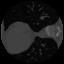
\includegraphics[width=\textwidth]{baseline_small_clean.png}
      \caption{Clean sinogram embedding with $k=2$}
      \label{fig:small_experiment_clean2}
  \end{subfigure}\hfill
  \begin{subfigure}[t]{0.3\textwidth}
    
\includegraphics[width=\textwidth]{random__graph_small_experiment.png}
    \caption{Reconstruction Erdős–Rényi input graph with $p=0.01$}
    \label{fig:small_experiment_random_graph}
  \end{subfigure}\hfill
  \begin{subfigure}[t]{0.3\textwidth}
    
\includegraphics[width=\textwidth]{knn__graph_small_experiment.png}
    \caption{Reconstruction k-NN input graph with $k=10$}
    \label{fig:small_experiment_knn_graph}
  \end{subfigure}
  \caption{Example image reconstructions for different input graphs.}
  \label{fig:input_graph_small}
\end{figure}



  \paragraph{Does result improve with more observations?}
  Yes.
  For this question to answer, multiple models have been trained for graphs with 512, 1024 and 2048 observations
  as well as different $k = (2,6,8,10,20)$.
  In Table~\ref{tab:graph_knn} results are presented, where results are averaged by number of observations 
  for different $k$.

  A larger number of nodes can improve the models. 
  But, training is also more expensive regarding execution time. 
  Therefore, for all upcoming experiments number of observations is fixed to 1024, as it looks like a good
  value in between, with good reconstruction result but also not too much training time.
  
  \begin{table}[H]
    \centering
      \begin{tabular}{l|ccc}
      \toprule
      \textbf{Number of observations} & \textbf{SNR} & \textbf{Loss} & \textbf{Training time (s)}  \\ 
      \midrule
      512  &  7.22    &  822.6  & 2678.6 s \\ \hline
      1024 &  7.80    &  766.88 & 4216.1 s \\ \hline
      2048 &  8.55    &  701.49 & 7609.0 s  \\ \hline
      \midrule
      \end{tabular}
    \caption{Loss and SNR for different number of observations, which refer to the average of 
    different k-NN parameters $k = (2,6,8,10,20)$.}
    \label{tab:graph_knn}
  \end{table}

  \paragraph{What is a good value for  $k$?}

  To find suitable $k$, multiple models have been trained with different $k=(1,2,3,4,6,8,10,20)$
  as well as different \snry (0 dB and -10 dB).

  In Table~\ref{tab:small_knn_snr} the results of evaluated models are presented.
  For \snry 0 dB the best result can be achieved with $k=2$ and for \snry -10 dB $k=1$.
  With our assumption of fixed angles, it looks like only a few neighbors are enough to capture 
  important information in the neighborhood.

  \begin{table}[H]
    \centering
    \begin{tabular}{c|cc|cc}
      \toprule
      \textbf{k-NN}         & \multicolumn{2}{c|}{\snrh{ 0}} & \multicolumn{2}{c}{\snrh{ -10}}  \\
      \textbf{parameter k}  & \textbf{SNR} & \textbf{Loss} & \textbf{SNR} & \textbf{Loss} \\ 
      \midrule
      1    & 8.81          & 678.67          & \textbf{7.09} & \textbf{827.51} \\ \hline
      2    & \textbf{9.16} & \textbf{652.38} & 6.95          & 849.44 \\ \hline
      3    & 8.64          & 689.15          & 6.38          & 912.73 \\ \hline
      4    & 8.37          & 712.44          & 6.29          & 906.75 \\ \hline
      6    & 8.25          & 722.81          & 5.81          & 958.32  \\ \hline
      8    & 7.99          & 744.07          & 5.64          & 985.81  \\ \hline
      10   & 7.30          & 804.70          & 5.54          & 996.25  \\ \hline
      20   & 6.30          & 910.45          & 4.82          & 1090.55 \\
      \midrule
    \end{tabular}
  
    \caption{Different k-NN values for \snry 0 dB and -10 dB }
    \label{tab:small_knn_snr}
  \end{table}

  

\subsection{GAT Experiments}
In this section, experiments are presented with focus on the GAT and its parameters.
Mainly, two parameters are important: number of heads and number of layers.

Therefore, number of layers is expected to keep rather low, as it defines the exposure of the k-hop neighborhood.
The dataset observations have only resolution 64x64 and consequently, it is expected that too many layers will 
average a too large neighborhood.

Further, number of heads determines if the learned weight matrix is divided into several parts.
The larger the number of heads, the smaller are the parts of the weight matrix.
Overall, larger number of heads is expected to smoothen denoising, but too large values
will divide weight matrix in too many parts, leading to bad results.

Experiments have been computed in parallel and results for k-NN have not been present before. 
Therefore, graphs were constructed with $k=8$, even tough it is not the best value for $k$.
Further, convolution was applied with a single channel, kernel size = 3 and padding 1.
As focus is on GAT parameters, U-Net was again omitted.
Further, multiple experiments with layers = $(2,3,4,6)$ and heads = $(1,2,4,8,16)$ have been evaluated, 
where results can be found in Table~\ref{tab:small_gat_results}.

\begin{table}[H]
  \centering
  \begin{tabular}{c|cc|cc|cc|cc|cc}
    \toprule
    \textbf{Heads} & \multicolumn{2}{c|}{\footnotesize \textbf{2 Layers}} & \multicolumn{2}{c|}{\footnotesize \textbf{3 Layers}} & \multicolumn{2}{c|}{\footnotesize \textbf{4 Layers}} & \multicolumn{2}{c|}{\footnotesize \textbf{6 Layers}} & \multicolumn{2}{c}{\footnotesize \textbf{Average}} \\
                   & \textbf{SNR} & \textbf{Loss} & \textbf{SNR} & \textbf{Loss} & \textbf{SNR} & \textbf{Loss} & \textbf{SNR} & \textbf{Loss} & \textbf{SNR} & \textbf{Loss} \\ 
    \midrule
    1    &  7.55	         & 784.23          & 6.65	          & 869.1          & \textbf{6.08}	& \textbf{934.2}  & 3.19	        & 1334.1          & 5.87 & 980.4 \\ \hline
    2    &  7.88	         & 753.4           & 7.17	          & 821.7          & 5.98	          & 958.8           & 3.55	        & 1256.5          & 6.15 & 947.6 \\ \hline
    4    &  8.22	         & 727.55          & 6.26	          & 927.4          & 4.10	          & 1176.1          & \textbf{4.08}	& \textbf{1191.2} & 5.67 & 1005.6 \\ \hline
    8    &  8.14 	         & 732.28          & \textbf{7.28}	& \textbf{808.1} & 5.54	          & 1010.4          & 2.81	        & 1516.2          & 5.94 & 1016.7 \\ \hline
    16   &  \textbf{8.27}  & \textbf{721.9}  & 5.69	          & 990.5          & 5.98	          & 941.8           & 2.81	        & 1516.0          & 5.66 & 1042.6 \\ \hline
    
    Average  &  8.01 & 743.9 & 6.59 & 883.4 & 5.54 & 1004.3 & 3.29 & 1362.8   \\ 
    \midrule
  \end{tabular}
  \caption{Models trained with different GAT parameters: best and average result in column is marked bold. }
  \label{tab:small_gat_results}
\end{table}


\paragraph{The more layers the better result?}
No. As expected, when working with too many layers, denoising starts failing as it averages over a
neighborhood, which is too large. In Table~\ref{tab:small_gat_results}, 6 layers clearly get the worst result,
followed by 4, 3 and 2 layers.

\paragraph{How does multiple heads affect result?}
It has an overall positive impact. 
During experiments, for every layer $l$ with single-head result, there is a better result for $l$, but multiple-heads. 
For 2 layers, single-head model performs with an average SNR of 7.55 dB where with 16 heads average SNR is 8.27.

2 layers seems to be most promising and number of heads 4 seems to be a reasonable choice for heads.
With 16 heads, the result was even a bit better. As 16 heads performed rather low for other number of layers, 
the best GAT parameters are considered to be 2 layers and 4 heads.
To make sure that $k=2$ is a good setting for these GAT parameters as well, the k-NN experiment
have been recomputed for 2 layers and 4 heads. Table~\ref{tab:small_knn_2} presents results, which 
give the same insight as for previous k-NN experiments.

\paragraph{How about some dropout?}
A small experiment with fixed network parameters
and different dropout values $(0, 0.01, 0.03, 0.05, 0.1)$ have been calculated. 
Results are presented in Figure~\ref{tab:small_droput}.
There is not too much of a difference, without dropout, model got the best value, followed by 
0.03 and 0.05 with almost the same result. 

Therefore, in future trainings, dropout of 0.05 was used.

\subsection{Convolution Experiments}

For convolution, kernel size and padding can be defined.
Moreover, it is possible to increase number of channels during convolution. 
For GAT, number of layers determine the averaging neighborhood.
As multiple channels are expected to perform better with multiple layers,
there could be a trade-off between GAT quality (size of averaging neighborhood) and convolution quality (increasing number of channels). 

First, some experiments with 4 layers and 2 heads have been executed with different number of kernel, padding and number of channels.
Noise was added to reach an SNR of -5 dB.
The aim is to find good convolution kernel and padding parameter value.

\paragraph{What is a good kernel size?}

In Table~\ref{tab:small_convolution} results are illustrated. 
Best results are achieved with only 1 channel and smallest kernel size of 3 with padding 1.
This is not too big of a surprise, observation dimension is only 64 and, therefore, a smaller kernel make sense.


\begin{table}[H]
  \centering
  \begin{tabular}{c|cc|cc|cc|cc}
    \toprule
    \textbf{Kernel}  & \multicolumn{2}{c|}{1 Channel} & \multicolumn{2}{c|}{4 Channel} & \multicolumn{2}{c|}{8 Channel} & \multicolumn{2}{c}{16 Channel} \\
    \textbf{and Padding}  & \textbf{SNR} & \textbf{Loss} & \textbf{SNR} & \textbf{Loss} & \textbf{SNR} & \textbf{Loss} & \textbf{SNR} & \textbf{Loss} \\ 
    \midrule
      7 / 3 & 3.56 & 1328.7                  & 4.60  &  1330.0                   & \textbf{3.76} & \textbf{1363.4} & \textbf{2.81}  & \textbf{1515.7} \\ \hline
      5 / 3 & 4.94 & 1081.0                  & 2.76  &  1548.5                   & 2.66 & 1597.0                   & \textbf{2.81}  & \textbf{1515.7} \\ \hline
      3 / 1 & \textbf{6.49} & \textbf{900.6} & \textbf{5.06}  &  \textbf{1084.8} & 1.30 & 2336.1                   & 0.05  & 2844.4 \\

    \midrule
  \end{tabular}

  \caption{Small experiment: Convolution for GAT-Denoiser with 4 layers and 2 heads}
  \label{tab:small_convolution}
\end{table}

\paragraph{Is there a trade-off between GAT and convolution quality?}

As kernel size of 3 with padding 1, seems to be a good value for the LoDoPaB-CT dataset, 
in the second convolution experiment different GAT architectures are compared with kernel size 3.
Good performing GAT architectures for layers 2 to 4 have been chosen: 2 layers with 4 heads, 3 layers with 8 heads
and 4 layers with 2 heads.

Resulting evaluation can be seen in Table~\ref{tab:small_convolution_2}.
Additionally, for every GAT architecture model without convolution was computed as well.
For every architecture, there was a model with convolution which performed better than the one without convolution.


\begin{tcolorbox}[colback=red!5!white,colframe=red!75!black]
  Convolution can be considered to contribute to the success of GAT-Denoiser.
\end{tcolorbox}



\begin{table}[H]
  \centering
  \begin{tabular}{l|cc|cc|cc}
    \toprule
    \textbf{Channels } & \multicolumn{2}{c|}{2 Layers} & \multicolumn{2}{c|}{3 Layers} & \multicolumn{2}{c}{4 Layers}  \\
                       & \textbf{SNR} & \textbf{Loss} & \textbf{SNR} & \textbf{Loss} & \textbf{SNR} & \textbf{Loss} \\ 
    \midrule
		No Conv & 6.99  & 839.3 & 4.31   & 1175.5 & \textbf{6.91} & \textbf{842.2}     \\ \hline
		1       & \textbf{8.10}  & \textbf{735.6} & 6.91   & \textbf{842.2} & 6.49 & 900.6     \\ \hline
		4       & 7.12  & 834.6 & 6.45   & 903.0 & 5.06 & 1084.8   \\ \hline
		8       & 7.79  & 767.3 & \textbf{7.01}   & 862.9 & 1.30 & 2336.1    \\ \hline
		16      & 7.45  & 798.8 & 5.97   & 1002.9 & 0.05  & 2844.4   \\
    \midrule
  \end{tabular}

  \caption{Small experiment: Convolution for GAT-Denoiser with different number of layers and heads}
  \label{tab:small_convolution_2}
\end{table}



\subsection{Loss Experiments}
An experiment was set up to compare $\mathcal{L}$ from Equation~\ref{eq:loss_reco} 
with $\mathcal{L}_{sino}$ from Equation~\ref{eq:loss_sino}.
The same network parameters have been used, but once loss during training was defined 
with $\mathcal{L}$ and once $\mathcal{L}_{sino}$. The experiment
have been computed for \snry 0, -5, -10 and -15 dB.

\paragraph{Is our end-to-end learning a good idea?}
Yes, but it comes with a price. 
Averaged results over training loss can be found in Table~\ref{tab:loss_sino_reco}. 
Overall, model trained with loss $\mathcal{L} $ performed around 1 dB in SNR better.
But, training of the network took much longer, more than factor 3. 
This is not a big surprise, as for learning with $\mathcal{L} $, reconstruction of every sample
needs to be done in every epoch, where for $\mathcal{L}_{sino}$ reconstruction can be omitted.

\begin{tcolorbox}[colback=red!5!white,colframe=red!75!black]
  End-to-end learning with loss $\mathcal{L} $ contributes to the success of GAT-Denoiser and 
   is used in further experiments.
\end{tcolorbox}


\begin{table}[H]
  \centering
    \begin{tabular}{l|ccc}
    \toprule
    \textbf{Loss training} & \textbf{Average SNR} & \textbf{Average Loss} & \textbf{Training time (s)}  \\ 
    \midrule
    $\mathcal{L} $         &  7.29    &  816.7  & 3812 s \\ \hline
    $\mathcal{L}_{sino}$   &  6.49    &  981.3  & 1209 s \\ \hline
    \midrule
    \end{tabular}
  \caption{Average Loss and SNR of different training loss $\mathcal{L}$ and $\mathcal{L}_{sino}$}
  \label{tab:loss_sino_reco}
\end{table}


\subsection{GAT-Denoiser Component Experiments}

The final small scale experiments aim to see contribution of the single components in action and 
to compare them.
Therefore, a fixed overall architecture is defined and experiments
with different combination of components (Convolution, GAT and U-Net) will be calculated.
Further, models with joint U-Net training have been evaluated.
The fixed settings for GAT-Denoiser have been defined with 2 layers, 4 heads, convolution with 
kernel size 3 and padding 1. $k$ was set to 2.
Overall, 8 models have been evaluated and compared against the baseline algorithms for  \snry $ = (-15,-10,-5,0) $ dB.

Results are plotted in Figure~\ref{fig:small_components} and numeric values can be found in Table~\ref{tab:small_gat_components}.
First, \textit{GAT} is the model, where no convolution and no U-Net is active. 
Second, \textit{GAT + Conv} refers to the model with GAT and convolution but no U-Net.
Additionally, the two models have been combined with U-Net, which are referred as 
\textit{GAT + U-Net} and \textit{Conv + GAT + U-Net}.
Last, models with joint U-Net training are presented.
\textit{U-Net*} denotes that during all 200 epochs, U-Net was jointly trained.
\textit{U-Net**} denotes that during the first 100 epochs, U-Net was kept static 
and training was activated for the second 100 epochs.

\ref{tab:small_gat_components}

\begin{figure}[H]
  \centering
  \label{fig:small_components}
  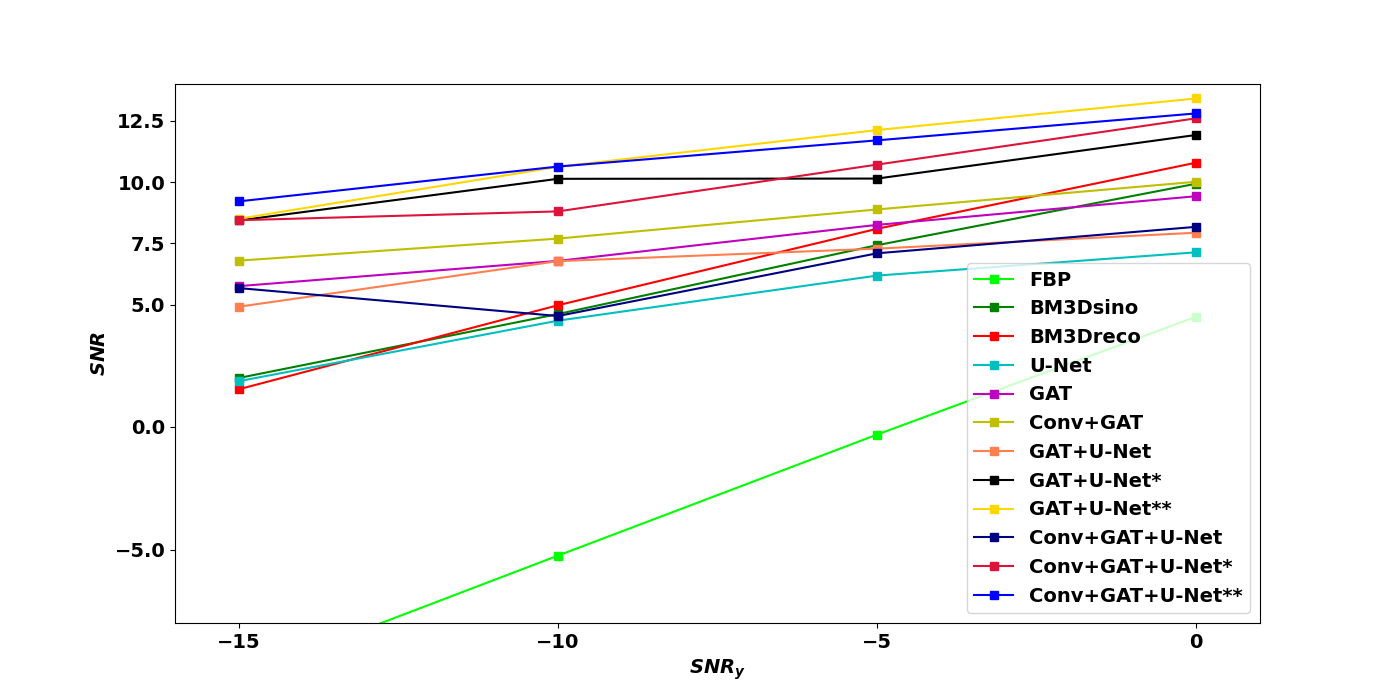
\includegraphics[width=0.9\textwidth]{small_components_result.png}
  \caption{
    Reconstruction SNR of different models and baseline algorithms.
    }
\end{figure}

Model \textit{GAT} is not able to beat baseline algorithms, and it seems that only applying GAT is not enough.
\textit{GAT + Conv} performs slightly better. When adding U-Net in the models \textit{GAT + U-Net} \textit{Conv + GAT + U-Net},
the visual results improve slightly but reconstruction SNR is still not able to beat baseline algorithms.
Finally, with joint training of GAT-Denoiser and U-Net, 
results can beat baseline algorithms for the small scale problem. It was helpful, to first train only GAT-Denoiser for 100 epochs 
and start joint training for the second 100 epochs.

Figure~\ref{fig:small_components_overview} illustrates visual results for all baseline algorithms and some GAT-Denoiser models.
Further, clean sample is presented in Figure~\ref{fig:small_clean_sample_overview}.

\begin{figure}[H]
  \captionsetup[subfigure]{justification=centering}
  \centering
  \begin{subfigure}[t]{0.16\textwidth}
    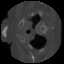
\includegraphics[width=\textwidth]{small/small_clean.png}
    \caption{Clean sample}
    \label{fig:small_clean_sample_overview}
  \end{subfigure} \hfill
  \begin{subfigure}[t]{0.16\textwidth}
    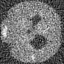
\includegraphics[width=\textwidth]{small/small_fbp.png}
    \caption{FBP}
  \end{subfigure} \hfill
  \begin{subfigure}[t]{0.16\textwidth}
    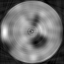
\includegraphics[width=\textwidth]{small/small_gat.png}
    \caption{\textit{GAT}}
  \end{subfigure} \hfill
  \begin{subfigure}[t]{0.16\textwidth}
    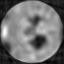
\includegraphics[width=\textwidth]{small/small_conv_gat.png}
    \caption{\textit{Conv+GAT}}
  \end{subfigure} \hfill
  \begin{subfigure}[t]{0.16\textwidth}
    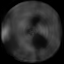
\includegraphics[width=\textwidth]{small/small_gat_unet.png}
    \caption{\textit{GAT + U-Net}}
  \end{subfigure}

  \begin{subfigure}[t]{0.16\textwidth}
    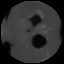
\includegraphics[width=\textwidth]{small/small_gat_unet_train.png}
    \caption{\textit{GAT + U-Net*}}
  \end{subfigure} \hfill
  \begin{subfigure}[t]{0.16\textwidth}
    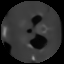
\includegraphics[width=\textwidth]{small/small_gat_unet_train_2.png}
    \caption{\textit{GAT + U-Net**}}
  \end{subfigure} \hfill
  \begin{subfigure}[t]{0.16\textwidth}
    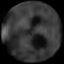
\includegraphics[width=\textwidth]{small/small_conv_gat_unet.png}
    \caption{\textit{Conv + GAT + U-Net}}
  \end{subfigure} \hfill
  \begin{subfigure}[t]{0.16\textwidth}
    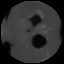
\includegraphics[width=\textwidth]{small/small_gat_unet_train.png}
    \caption{\textit{Conv + GAT + U-Net*}}
  \end{subfigure} \hfill
  \begin{subfigure}[t]{0.16\textwidth}
    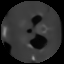
\includegraphics[width=\textwidth]{small/small_gat_unet_train_2.png}
    \caption{\textit{Conv + GAT + U-Net**}}
  \end{subfigure}
  \caption{Sample reconstruction for small scale GAT-Denoiser models \snry 0 dB}
  \label{fig:small_components_overview}
\end{figure}

\section{Large scale Experiments}

In this section, large scale experiments are presented, which have been trained on the complete LoDoPaB-CT dataset
as well as evaluated on the complete LoDoPaB-CT test dataset.
From last section, the most promising parameters for the GAT-Denoiser architecture have been chosen
to find the best model. The following parameters have been fixed during the large scale experiments:
$k=2$, number of layers = 2, number of heads = 4, convolution with kernel size 3 and padding 1.
The GAT-Denoiser have been trained for 20 epochs, if not mentioned differently.


\subsection{Baseline}
In Table~\ref{tab:baseline-large}, baseline results for large experiment can be found.
As only the number of samples changed, but algorithms are fixed, the result is roughly 
the same as for the small scale experiments.

\subsection{GAT-Denoiser Components Experiments}
The main components of the GAT-Denoiser pipeline have been tested with different models.
As a result of the small scale experiments, jointly training U-Net was most promising, 
when there was first some training on GAT-Denoiser solely and in a second part a joint training phase.
Therefore, model {Conv + GAT + U-Net*} and {GAT + U-Net*} is omitted for the large scale experiments.
Moreover, {... U-Net**} denotes that models have been first trained 10 epochs without
U-Net training and then 10 epochs with U-Net training.


\begin{figure}[H]
  \centering
  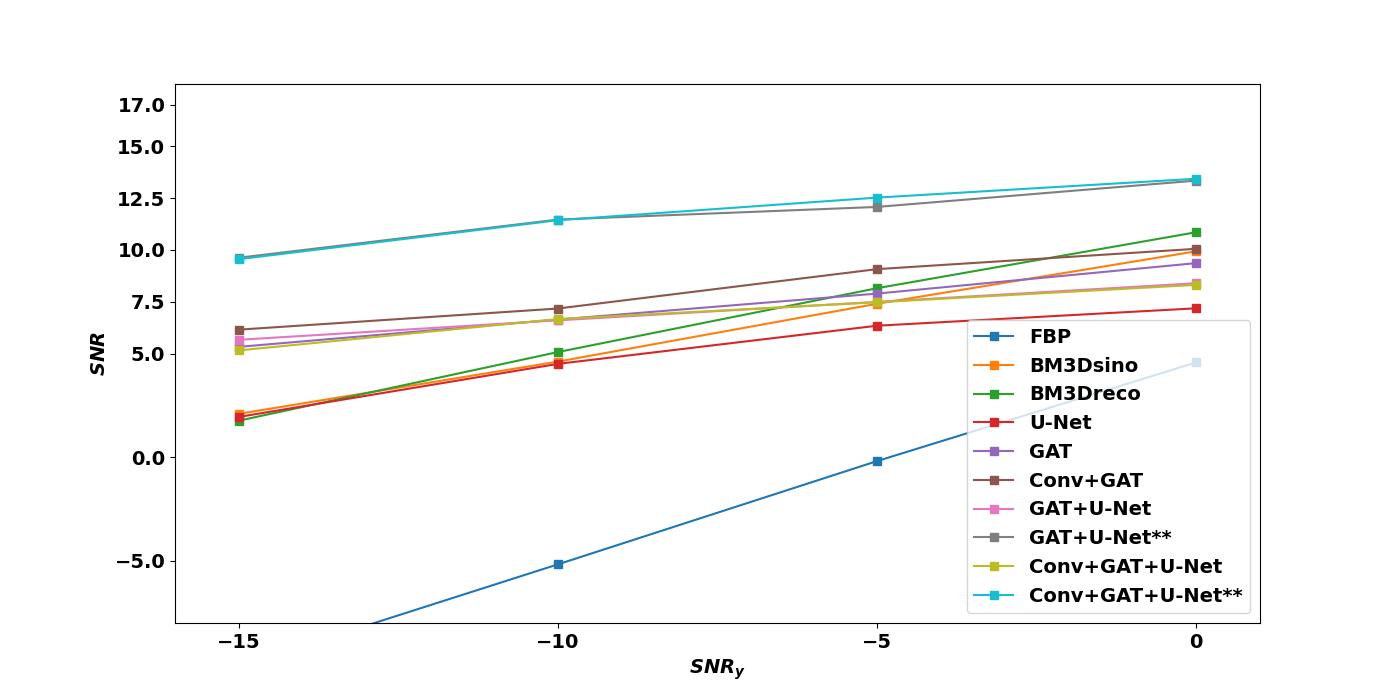
\includegraphics[width=0.8\textwidth]{large_components_result.png}
  \caption{Resulting SNR of different models and baseline algorithms.}
  \label{fig:large_components}
\end{figure}

Figure~\ref{fig:large_components} presents resulting SNR for baseline algorithms and 
different GAT-Denoiser models. Further, numerical results are presented in Table~\ref{tab:large_gat_components_knn2}
The results are rather similar compared to the small scale experiments.
Overall reconstruction is slightly better, as during training more samples have been seen.
Again, approaches with joint U-Net and GAT-Denoiser training results best.

\subsection{Best Models Experiments}
For the most promising architectures, the one with joint U-Net and GAT-Denoiser training,
the models have been further trained for another 20 epochs. 
In Table~\ref{tab:large_best_models} final results are illustrated. 
The number in brackets denotes the number of training epochs without U-Net followed by
the number of epochs with joint model training.

All in all, the few more epochs could sometimes improve result, as for \textit{Conv + GAT + U-Net} and \snry 0 dB.
Although, this is not always the case and in some scenarios, the model even performed worse, as for 
\textit{GAT + U-Net} and \snry -10 dB.


\begin{table}[H]
  \centering
  \begin{tabular}{l|cc|cc|cc|cc}
    \toprule
    \textbf{Model} & \multicolumn{2}{c|}{\snrh{ 0}} & \multicolumn{2}{c|}{\snrh{ -5}} & \multicolumn{2}{c|}{\snrh{ -10}} & \multicolumn{2}{c}{\snrh{ -15}} \\
                       & \textbf{SNR} & \textbf{Loss} & \textbf{SNR} & \textbf{Loss} & \textbf{SNR} & \textbf{Loss} & \textbf{SNR} & \textbf{Loss} \\ 
    \midrule

    GAT+U-Net(10/10)          & 13.34           & 413.8          & 12.07          & 469.2          & \textbf{11.46} & \textbf{502.0} & 9.62 & 633.5 \\ \hline
    GAT+U-Net(10/30)          & \textbf{13.43}  & \textbf{406.2} & \textbf{12.85} & \textbf{428.2} & 10.83 & 546.2                   & 9.65 & \textbf{603.34} \\ \hline
    GAT+U-Net(20/20)          & 13.16           & 412.2          & 12.10          & 469.9          & 11.02 & 529.0                   & \textbf{10.03} & 606.0 \\ \hline
    Conv+GAT+U-Net(10/10)   & 13.43           & 403.5          & 12.52          & 450.1          & \textbf{11.43} & 509.9          & 9.55 & 638.0 \\ \hline
    Conv+GAT+U-Net(10/30)   & 13.68           & 395.4          & 12.32          & 460.3          & 11.40 & \textbf{509.1}          & 9.25 & 688.1 \\ \hline
    Conv+GAT+U-Net(20/20)   & \textbf{13.87}  & \textbf{385.4} & \textbf{12.81} & \textbf{442.3} & 10.90 & 547.5                   & \textbf{10.1} & \textbf{604.4} \\ 

    \midrule
  \end{tabular}
  \caption{Baseline results large experiments}
  \label{tab:large_best_models}
\end{table}

A single sample reconstruction for \snry 0 dB is presented in Figure~\ref{fig:large_scale_best_reco}.
Additional visual results are presented in the Appendix~\ref{sec:large_scale_visual_results} for baseline algorithms 
and the best performing large scale GAT-Denoiser models for different $\textit{SNR}_y$. 

\begin{figure}[H]
  \captionsetup[subfigure]{justification=centering}
  \centering
  \begin{subfigure}[t]{0.16\textwidth}
    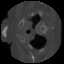
\includegraphics[width=\textwidth]{large/large_clean.png}
    \caption{Clean sample}
  \end{subfigure}
  \begin{subfigure}[t]{0.16\textwidth}
    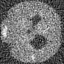
\includegraphics[width=\textwidth]{large/large_fbp.png}
    \caption{FBP}
  \end{subfigure}
  \begin{subfigure}[t]{0.16\textwidth}
    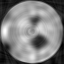
\includegraphics[width=\textwidth]{large/large_gat.png}
    \caption{\textit{GAT}}
  \end{subfigure}
  \begin{subfigure}[t]{0.16\textwidth}
    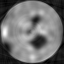
\includegraphics[width=\textwidth]{large/large_conv_gat.png}
    \caption{\textit{Conv+GAT}}
  \end{subfigure}
  \begin{subfigure}[t]{0.16\textwidth}
    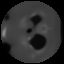
\includegraphics[width=\textwidth]{large/large_gat_unet_train_best.png}
    \caption{\textit{GAT+U-Net(10/30)}}
  \end{subfigure}
  \begin{subfigure}[t]{0.16\textwidth}
    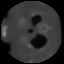
\includegraphics[width=\textwidth]{large/large_conv_gat_unet_train_best.png}
    \caption{\textit{Conv+GAT+U-Net(20/20)}}
  \end{subfigure}
  \caption{Large scale experiments visual results.}
  \label{fig:large_scale_best_reco}
\end{figure}

